\section{Teoria della Probabilitá}
    \subsection{Introduzione}
        Perché abbiamo bisogno della teoria della probabilitá? Prendiamo un sistema di comunicazione:
        \begin{figure}[H]
            \centering
                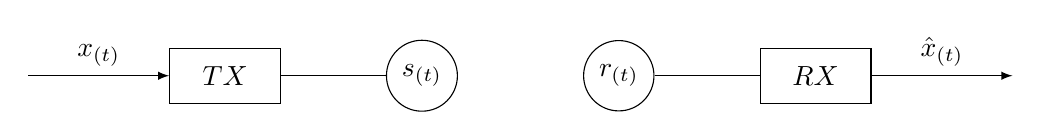
\begin{tikzpicture}[
                        node distance=2.5cm,
                        >=latex
                    ]
                    % Blocks
                    \node [coordinate] (input) {};
                    \node [rectangle, draw,minimum height=2em, minimum width=4em,right of=input] (TX) {$TX$};
                    \node [circle,draw,right of=TX] (TXant) {$s_{(t)}$};
                    \node [circle,draw,right of=TXant] (RXant) {$r_{(t)}$};
                    \node [rectangle, draw,minimum height=2em, minimum width=4em,right of=RXant] (RX) {$RX$};
                    \node [coordinate,right of=RX] (output) {};
                
                    % Connections
                    \draw [->] (input) --node[above]{$x_{(t)}$} (TX);
                    \draw [-] (TX) -- (TXant);
                    \draw [-] (RXant) -- (RX);
                    \draw [->] (RX) --node[above]{$\hat{x}_{(t)}$} (output);
                \end{tikzpicture}    
            \label{fig:Sistema di comunicazione}
            \caption{Esempio sistema di comunicazione}
        \end{figure}
        Analizziamo la parte di trasmissione $TX$:
        \begin{figure}[H]
            \centering
                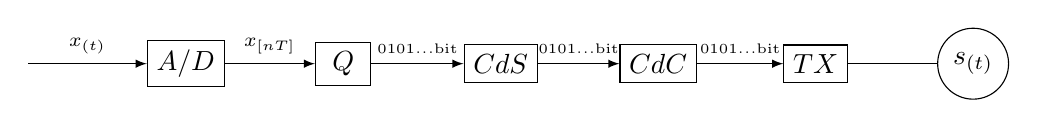
\begin{tikzpicture}[
                        node distance=2cm,
                        >=latex
                    ]
                    % Blocks
                    \node [coordinate] (input) {};
                    \node [rectangle, draw,minimum height=1em, minimum width=2em,right of=input] (AD) {$A/D$};
                    \node [rectangle, draw,minimum height=1em, minimum width=2em,right of=AD] (Q) {$Q$};
                    \node [rectangle, draw,minimum height=1em, minimum width=2em,right of=Q] (CS) {$CdS$};
                    \node [rectangle, draw,minimum height=1em, minimum width=2em,right of=CS] (CC) {$CdC$};
                    \node [rectangle, draw,minimum height=1em, minimum width=2em,right of=CC] (TX) {$TX$};
                    \node [circle,draw,right of=TX] (TXant) {$s_{(t)}$};
                
                    % Connections
                    \draw [->] (input) --node[above]{\scriptsize $x_{(t)}$} (AD);
                    \draw [->] (AD) --node[above]{\scriptsize$x_{[nT]}$} (Q);
                    \draw [->] (Q) --node[above]{\tiny$0101...$bit} (CS);
                    \draw [->] (CS) --node[above]{\tiny$0101...$bit} (CC);
                    \draw [->] (CC) --node[above]{\tiny$0101...$bit} (TX);
                    \draw [-] (TX) -- (TXant);
                \end{tikzpicture}    
            \label{fig:Sistema di comunicazione trasmettitore}
            \caption{Esempio sistema di trasmettitore}
        \end{figure}
        \begin{itemize}
            \item {Convertitore Analogico/Digitale ($A/D$): Campiona con frequenza $f_s$ e crea la sequenza $x_{[nT]}$.}
            \item {Quantizzatore ($Q$): Converte i valori della sequenza $x_{[nT]}$ in informazioni, bit. Ho sempre perdita di informazione a 
                questo livello, per quanti livelli di quantizzazione io metta il quantizzatore introdurrá sempre un'approssimazione. 
            }
            \item{Nei blocchi sotto elencati é dove entra in gioco la Teoria dei Codici, ci permettono di comprimere i dati e proteggerli dagli errori del canale:
                \begin{itemize}
                    \item {Codici di Sorgente ($CdS$): Comprimono i bit in ingresso dal quantizzatore eliminando la ridondanza.}
                    \item {Codifica di Canale ($CdC$): Aggiunge ridondanza ai dati da trasmettere per proteggere i dati dagli errori del canale.}
                \end{itemize}
            \item {Trasmettitore ($TX$):Si occupa di rendere il segnale trasmissibile sul canale di interesse e trasmettere il risultato $s_{(t)}$.}
            }
        \end{itemize}
        Analizziamo la parte di Ricezione $RX$:
        \begin{figure}[H]
            \centering
                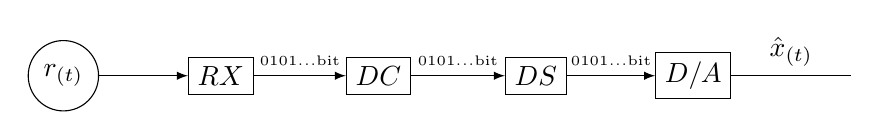
\begin{tikzpicture}[
                        node distance=2cm,
                        >=latex
                    ]
                    % Blocks
                    \node [circle,draw] (RXant) {$r_{(t)}$};
                    \node [rectangle, draw,minimum height=1em, minimum width=2em,right of=RXant] (RX) {$RX$};
                    \node [rectangle, draw,minimum height=1em, minimum width=2em,right of=RX] (DC) {$DC$};
                    \node [rectangle, draw,minimum height=1em, minimum width=2em,right of=DC] (DS) {$DS$};
                    \node [rectangle, draw,minimum height=1em, minimum width=2em,right of=DS] (DA) {$D/A$};
                    \node [coordinate,right of = DA] (output) {};
                
                    % Connections
                    \draw [->] (RXant) --node[above]{} (RX);
                    \draw [->] (RX) --node[above]{\tiny$0101...$bit} (DC);
                    \draw [->] (DC) --node[above]{\tiny$0101...$bit} (DS);
                    \draw [->] (DS) --node[above]{\tiny$0101...$bit} (DA);
                    \draw [-] (DA) --node[above]{$\hat{x}_{(t)}$} (output);
                \end{tikzpicture}    
            \label{fig:Sistema di comunicazione ricevitore}
            \caption{Esempio sistema di ricevitore}
        \end{figure}
        \begin{itemize}
            \item {RIcevitore ($RX$): Si occupa della ricezione del segnale trasmesso $r_{(t)}$.}
            \item{La Teoria dei Codici si applica anche in ricezione per la decodifica:
                \begin{itemize}
                    \item {Decodifica Canale ($DC$): .}
                    \item {Decodifica Sorgente($DS$): .}
                \end{itemize}
            }
            \item {Convertitore Digitale/Analogico ($D/A$): Ricostruisce il segnale $\hat{x}_{(t)}$. 
            }
        \end{itemize}
        Analizziamo il canale di trasmissione:
        \begin{figure}[H]
            \centering
                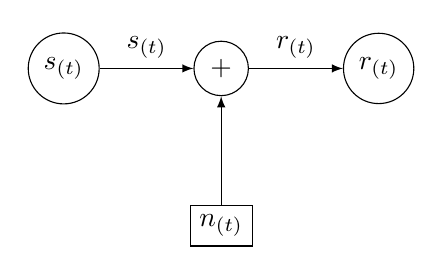
\begin{tikzpicture}[
                        node distance=2cm,
                        >=latex
                    ]
                    % Blocks
                    \node [circle,draw] (TXant) {$s_{(t)}$};
                    \node [circle, draw,right of=TXant] (sum) {$+$};
                    \node [rectangle, draw,below of = sum,minimum height=1em, minimum width=2em] (error) {$n_{(t)}$};
                    \node [circle,draw,right of=sum] (RXant) {$r_{(t)}$};
                
                    % Connections
                    \draw [->] (TXant) --node[above]{$s_{(t)}$} (sum);
                    \draw [->] (sum) --node[above]{$r_{(t)}$} (RXant);
                    \draw [->] (error) -- (sum);
                \end{tikzpicture}    
            \label{fig:Sistema di comunicazione canale con errore}
            \caption{Esempio sistema di canale con errore}
        \end{figure}
        Durante la trasmissione di $s_{(t)}$ viene introdotto dell'errore $n_{(t)}$. $n_{(t)}$ é un segnale completamente aleatorio di varia 
        natura:
        \begin{itemize}
            \item {Termico}
            \item {Interferenze}
            \item {Fading}
            \item {\dots}
        \end{itemize}
        \noindent di conseguenza $r_{(t)} = s_{(t)}+e_{(t)}$ diventa un segnale aleatorio.

        I segnali che analizzo sono tutte quantitá aleatorie: ho bisogno della probabilitá per analizzare la tipologia di segnali, anche per la sorgente
        potrei averne bisogno se non sono nel caso di segnali deterministici.

        \subsubsection{Tipi di modelli matematici}
            Esistono vari tipi di modelli matematici:
            \begin{itemize}
                \item {Deterministico: se esiste certezza e ne possiamo calcolare il valore a ogni istante del tempo (Es. sistemi lineari tempo invarianti)}
                \item {Probabilistico (Aleatorio): se non conosciamo la certezza con cui l'evento puó verificaris ma ne possiamo dare una valutazione probabilistica.}
            \end{itemize}
            Introduciam oquind i
    \subsection{Algebra dei Set (insiemi)}
        Un set é una collezione di elementi che condividono un criterio oggettivo per decidere se appartengono al set o no. Prendiamo come set $A$ e come 
        elemento del set $A$ $x$:
        \begin{itemize}
            \item {Se l'elemento appartiene al set: $x\in A$, veceversa se non appartiene:$x\notin A$}
            \item {Se un set é vuoto: $A=\{\emptyset\}=\emptyset$}
            \item {Se $x_1, \dots, x_n$ sono elementi di $A$ allora:
                \[
                    A=\{x_1, \dots, x_n \}
                \]
            }
        \end{itemize}
        \subsubsection{Operazioni booleane su set}
            \begin{itemize}
                \item {Unione ($A\cup B$): l'unione di due set $A$ e $B$ é a sua volta un set composto dagli elementi che appartegono a $A$ o $B$, o entrambi.}
                \item {Intersezione ($A\cap B$): l'intersezione di due set $A$ e $B$ é a sua volta un set composto dagli elementi che appartegono a $A$ e $B$.
                \begin{figure}[H]
                    \centering
                    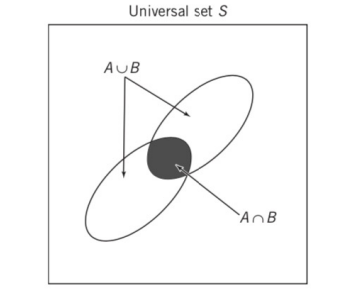
\includegraphics[width = 5cm]{media/Unione_Intersezione.png}
                    \caption{Unione e Intersezione} 
                \end{figure}
                }
                \item {Disgiunzione: é una relazione tra due set $A$ e $B$, essi sono disgiunti se tra loro non hanno elementi comuni ($A\cap B = \emptyset $).}
                \item {Partizione ($A = A_1\cup A_2\cup A_3$): la partizione di un insieme $A$ é una divisione dell'insieme stesso in subset disgiunti.
                \begin{figure}[H]
                    \centering
                    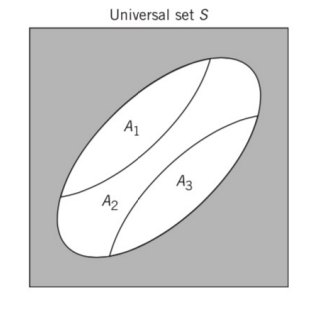
\includegraphics[width = 5cm]{media/Insiemi_distinti.png}
                    \caption{Disgiunzione e Partizione} 
                \end{figure}
                }
                \item {Complemento ($A^c$): dati due set $A$ e $B:A\subset B$ il complemento del set $A$ é il set contenente gli elementi di $B$ non appartenenti ad $A$.
                \begin{figure}[H]
                    \centering
                    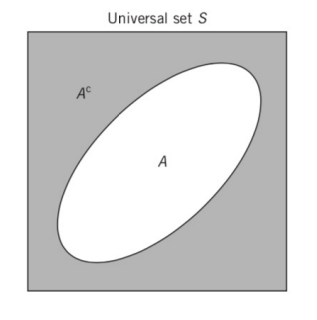
\includegraphics[width = 5cm]{media/Insieme_Complementare.png}
                    \caption{Complemento}
                \end{figure}
                }
            \end{itemize}
        \subsubsection{Operazioni algebriche su set}
            \begin{itemize}
                \item {Idempotenza
                    \[
                        \left(A^c\right)^c = A
                    \]
                }
                \item {Propietá commutativa
                    \begin{gather}
                        A\cup B = B\cup A \nonumber \\
                        A\cap B = B\cap A \nonumber
                    \end{gather}
                }
                \item {Propietá associativa
                    \begin{gather}
                        (A\cup B) \cup C= (A\cup C)\cup B \nonumber \\
                        (A\cap B) \cap C= (A\cap C)\cap B \nonumber                        
                    \end{gather}
                }
                \item {Propietá distributiva
                    \begin{gather}
                        (A\cup B) \cap C= (A\cap C)\cup (B \cap C) \nonumber \\
                        (A\cap B) \cup C= (A\cup C)\cap (B \cup C) \nonumber                        
                    \end{gather}
                }
            \end{itemize}

    \subsection{Modelli probabilistici}
        La descrizione di un esperimento con risultati incerti é chiamato \emph{modello probabilistico}, la costruzione del modello richiede:
        \begin{itemize}
            \item {Spazio dei campioni o set universale $S$: nel quale sono presenti tutti i possibili risultati dell'esperimento.}
            \item {Una classe di eventi $A$ che sia un subset di $S$.}
            \item {Legge della Probabilitá: alla quale una quantitá non negativa $P[A]$ viene assegnata ad $A$. $P[A]$ viene detta probabilitá dell'evento $A$: rappresenta
                con quale occorrenza potrebbe verificarsi il risultato delĺ'esperimento $A$.}
        \end{itemize}
        \begin{figure}[H]
            \centering
            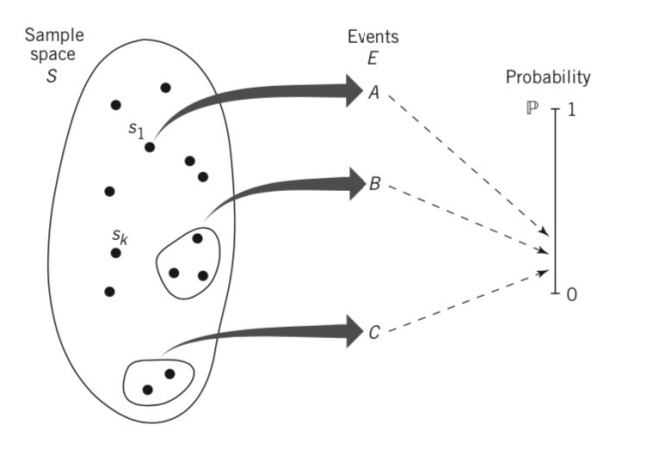
\includegraphics[width = 5cm]{media/Insieme_probabilita.png}
            \caption{Modello Probabilistico} 
        \end{figure}
        Un evento puó avere come risultato un singolo risultato o un subset di risultati di $S$.
        \subsubsection{Assiomi della probabilitá}
            \begin{enumerate}
                \item \label{Ass. Prob. 1}{Non Negativitá: la probabilitá di $A$ é un numero non negativo:
                    \[
                        0\leq P[A] \leq 1,\ \forall \text{ evento A}
                    \]
                }
                \item \label{Ass. Prob. 2}{Additivitá: se $A$ e $B$ sono due eventi disgiunti, allora la probablitá dell'unione é: 
                    \[
                        P[A\cup B] = P[A] + P[B] 
                    \]
                }
                \item \label{Ass. Prob. 3}{Normalizzazione: la probabilitá del set universale $S$ é $P[S] = 1$}
            \end{enumerate}
            Si sviluppano alcune propietá della probabilitá:
            \begin{itemize}
                \item {
                    La probabilitá di un evento impossibile é zero.
                    Dimostrazione:
                }
                \item {
                    $P[A^c] = 1-P[A]$
                    Dimostrazione:
                }
                \item {
                    Se un evento $A$ é un subset di un evento $B$ allora: $P[A]\leq P[B]$. 
                    Dimostrazione: 
                }
                \item {
                    \begin{sloppypar}
                        Se due eventi $A$ e $B$ non sono disgiunti allora: ${P[A \cup B]= P[A] + P[B] -  P[A\cap B]}$\\
                        Dimostrazione:
                    \end{sloppypar}
                }
            \end{itemize}
        \subsubsection{Probabilitá condizionata}\label{Probabilitá condizionata}
            Prendiamo in esempio un esperimento che implica due eventi $A$ e $B$: $P[A|B]$ sia la probabilitá che un evento $A$ si verifichi
            dato il verificarsi dell'evento $B$, $P[A|B]$ é detta probabilitá condizionata di $A$ dato $B$, assumendo $P[B]\neq 0$:
            \[
                P[A|B] = \frac{P[A\cap B]}{P[B]}
            \]

        \subsubsection{Regola di Bayes}\label{Regola di Bayes}
            Supponiamo che si possano ricavare facilmente le probabilitá $P[A|B]$, $P[A]$ e $P[B]$ e vogliamo trovare la probabilitá condizionata $P[B|A]$:
            \[
                P[B|A] = \frac{P[A|B]P[B]}{P[A]}   
            \]
        \subsubsection{Indipendenza}\label{Indipendenza}
            Supponiamo che l'occorrenza  di un evento $A$ non fornisca nessuna informazione sull'evento $B$, $P[B|A] = 0$. Dalla regola di Bayes abbiamo $P[A|B] = P[A]$,
            i due eventi sono indipendenti e occorre che:
            \[
                P[A\cap B] = P[A]P[B]    
            \]
        \subsubsection{Legge della probabilitá totale}\label{Legge della probabilitá totale}
            Supponiamo $\{ A_n = 1,\dots N\}$ é un insieme di eventi disgiunti:

            \begin{figure}[H]
                \centering
                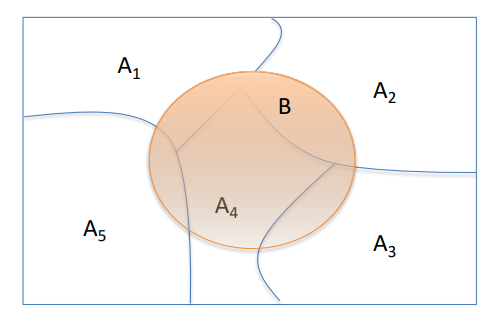
\includegraphics[width = 5cm]{media/probabilita_totale.png}
            \end{figure}
            \[
                P[B] = \sum_{n=1}^{N}P[B\cap A_n]    
            \]
        \subsubsection{Problemi esempio:}
            \paragraph{Radar Detection Problem:} Nel problema del rilevamento vogliamo analizzare in particolere tre tipi di probabilitá:
                \begin{itemize}
                    \item {
                        \emph{Probabilitá a priori} $P[A]$: probabilitá che il bersaglio sia nell'area.
                    }
                    \item {
                        \emph{Probabilitá di rivelazione} $P[B|A]$: probabilitá che il radar riveli il bersaglio, quando effettivamente il bersaglio
                         é presente nell'area.
                    }
                    \item {
                        \emph{Probabilitá di falso allarme} $P[B|A^c]$: probabilitá che il radar riveli il bersaglio, ma il bersaglio non
                         é effettivamente presente nell'area. 
                    }
                \end{itemize}
                Dati i dati delle relative probabilitá:
                \begin{gather}
                    P[A] = 0.02 \nonumber \\
                    P[B|A] = 0.99 \nonumber \\
                    P[B|A^c] = 0.01 \nonumber 
                \end{gather}
                $A^c$ indica che il bersagli non é presente. Il problema richiede di calcolare la probabilitá condizionata
                $P[A|B]$, la quale definisce la probabilitá che il bersaglio sia presente nell'area e il radar l'abbia rivelata.
                Soluzione:
                \[
                    \overset{\ref{Regola di Bayes}}{\Rightarrow} P[A|B] = \frac{P[A]P[B|A]}{P[B]}    
                \]                    
                Devo solo calcolare $P[B]$:
                \begin{align}
                        \overset{\ref{Legge della probabilitá totale}}{\Rightarrow} P[B] &= \sum_{n=1}^{2} P[B\cap A_n] = \sum_{n=1}^{2} P[B|A_n] P[A_n] \nonumber \\
                        P[B] &= P[B|A]P[A] + P[B|A^c]P[A^c] \nonumber \\
                             &= 0.99\dotproduct 0.02 + 0.01 \dotproduct 0.098 = 0.0296 \cong 0.03  \nonumber       
                \end{align}

                Ricordiamo che $P[A^c] = 1-P[A]$, nel nostro caso il problema ri risolve facilmente applicando il Th della probabilitá totale su due set disgiunti 
                $A$ e $A^c$. Possiamo quindi calcolare la probabilitá condizionata:
                \[
                    P[A|B] = \frac{P[A]P[B|A]}{P[B]} = \frac{0.02 \dotproduct 0.99}{0.03} = 0.66    
                \]

            \paragraph{Communication Problem:} In un sistema di comunicazione ho:
                \begin{itemize}
                    \item {$1$ é trasmesso con probabilitá $P[1] = 0.3$ e $0$ con probabilitá $P[0] = 1-P[1] = 0.7$}
                    \item {la probabilitá di errore é $P_e = 0.01$}
                \end{itemize}
                Richiesta: assumendo che venga ricevuto $0$, calcolare la probabilitá che questo sia stato effettivamente trasmesso.
                Soluzione: Definiamo i set di interesse:
                \begin{itemize}
                    \item {$A = \{0\text{ é stato trasmesso}\},\ A^c = \{1 \text{ é stato trasmesso}\}$}
                    \item {$B = \{0\text{ é stato ricevuto}\},\ B^c = \{1 \text{ é stato ricevuto}\}$}
                \end{itemize}
                \[
                    \overset{\ref{Regola di Bayes}}{\Rightarrow} P[A|B] = \frac{P[A]P[B|A]}{P[B]}    
                \]                           
                $P[B|A]$ non é altro che il probabilitá di corretta ricezione ($P[c]$), posso calcolarla dalla probabilitá di errore:
                \begin{gather}
                    P[e] = P[B^c|A] = P[B|A^c] = 0.01, \text{ probabilitá di errore} \nonumber \\
                    P[c] = P[B|A] = P[B^c|A^c] = 1-P[e]= 0.99, \text{ probabilitá di corretta ricezione}\nonumber 
                \end{gather}
                Calcoliamo $P[B]$:
                \begin{align}
                    \overset{\ref{Legge della probabilitá totale}}{\Rightarrow} P[B] &= \sum_{n=1}^{2} P[B\cap A_n] = \sum_{n=1}^{2} P[B|A_n] P[A_n] \nonumber \\
                    P[B] &= P[B|A]P[A] + P[B|A^c]P[A^c] \nonumber \\
                         &= 0.99\dotproduct 0.7 + 0.01 \dotproduct 0.3 = 0.696 \nonumber       
                \end{align}
                Possiamo quindi calcolare la probabilitá condizionata:
                \[
                    P[A|B] = \frac{P[A]P[B|A]}{P[B]} = \frac{0.7 \dotproduct 0.99}{0.696} = 0.995    
                \]
            \paragraph{Esempio palline:}
                Eventi: Pesco una pallina dall'urna \emph{pippo} e la metto nell'urna \emph{pluto}, infine pesco una pallina dall'urna \emph{pluto}.
                Calcolare la probabilitá di pescare una pallina bianca dall'urna \emph{pluto} ($P[\text{pesco 1 bianca da \emph{pluto}}] = P[A]$).  
                \begin{figure}[H]
                    \centering
                    
\includegraphics[width = 4cm]{media/uwu.png}
                \end{figure}
                Definiamo per prima cosa i set del problema:
                \begin{itemize}
                    \item {$A = \{ pesco una pallina bianca da pluto\}$}
                    \item {$B = \{ pesco una pallina bianca da pippo\}$}
                    \item {$B^c = C = \{ pesco una pallina nera da pippo\}$}
                \end{itemize}
                Calcoliamo $P[A]$:
                \begin{align}
                    \overset{\ref{Legge della probabilitá totale}}{\Rightarrow} P[A] &= \sum_{n=1}^{2} P[A\cap B_n] = \sum_{n=1}^{2} P[A|B_n] P[B_n] \nonumber \\
                    P[A] &= P[A|B]P[B] + P[A|C]P[C] \nonumber \\
                         &= \frac{3}{4}\frac{2}{3} + \frac{2}{4}\frac{1}{3} = \frac{2}{3}  \nonumber       
                \end{align}
                \begin{itemize}
                    \item {$P[A|B]$: pesco bianco da \emph{pluto} avendo inserito una bianca da \emph{pippo}}
                    \item {$P[A|C]$: pesco bianco da \emph{pluto} avendo inserito una nera da \emph{pippo}}
                \end{itemize}

                \subparagraph{Aggiungiamo due palline da \emph{pippo} in \emph{pluto}:} Cambia il Th della probabilitá totale:
                    \begin{itemize}
                        \item {$P[B]$: pesco due bianche da \emph{pippo} $= \frac{2}{3}\dotproduct \frac{1}{2} $}
                        \item {$P[A|B]$: pesco due bianche da \emph{pluto} avendo inserito due bianche da \emph{pippo}$= \frac{4}{5} $}
                        \item {$P[C]$: pesco una bianca e una nera da \emph{pippo} $= \frac{2}{3}\dotproduct \frac{1}{2} $}
                        \item {$P[A|C]$: pesco bianco da \emph{pluto} avendo inserito una bianca e una nera da \emph{pippo} $= \frac{3}{5} $}
                        \item {$P[D]$: pesco due nere da \emph{pippo}, é un evento impossibile $P[D] = 0$}
                        \item {$P[A|D]$: pesco bianco da \emph{pluto} avendo inserito due nere da \emph{pippo} $P[D] = 0$}
                        \item {$P[E]$: una nera e una bianca da \emph{pippo}$= \frac{1}{3}\dotproduct 1 $}
                        \item {$P[A|E]$: pesco bianco da \emph{pluto} avendo inserito una nera e una bianca da \emph{pippo} $= \frac{3}{5} $}
                    \end{itemize}
                    \begin{align}
                        \overset{\ref{Legge della probabilitá totale}}{\Rightarrow} P[A] &= \sum_{n=1}^{4} P[A\cap B_n] = \sum_{n=1}^{4} P[A|B_n] P[B_n] \nonumber \\
                        P[A] &= P[A|B]P[B] + P[A|C]P[C]+ P[A|D]P[D]+ P[A|E]P[E] \nonumber \\
                        &= \frac{4}{5}\frac{1}{3} + \frac{3}{5}\frac{1}{3} + 0 + \frac{3}{5}\frac{1}{3} = \frac{10}{15}  \nonumber       
                    \end{align}
        \subsubsection{Coefficiente binomiale}\label{Coefficiente binomiale}
            Il coefficiente binomiale $\binom{n}{k}$ é un numero intero non negativo che fornisce le combiazioni semplici di $n$ elementi di classe $k$,
            definito da:
            \[
                \binom{n}{k} = C(n;k) = \frac{n!}{k!\dotproduct n-k!}
            \]
            Possiamo usarli per calcolare la probabilitá di errore su eventi ripetuti inunione con la distribuzione di bernulli \ref{Probabilita di errore BSC}.
            \paragraph{Esempio su sistema di comunicazione binario:}
                Prendiamo in esempio un trasmettitore di codice binario a ripetizione con $R = \frac{1}{3}
                \begin{cases}
                    0 = [000]\nonumber \\
                    1 = [111]\nonumber    
                \end{cases}$. Calcolare la probabilitá di errore del sistema, $P[E]$, sapendo che la probabilitá di errore sul
                bit é $P[e] = 0.01$.
                Soluzione:
                Scelgo la mia regola di decisione per la decodifica dei bit, a maggioranza:
                \begin{gather}
                    1 \rightarrow \text{Se ho la maggioranza di uno nel codice, nel nostro caso 2 su 3} \nonumber \\
                    0 \rightarrow \text{Se ho la maggioranza di zero nel codice, nel nostro caso 2 su 3} \nonumber
                \end{gather}
                sbaglio il codice in trasmissione se ho sbagliato tre o due bit. Calcoliamo la probabilitá del canale,
                $P[E] \overset{\ref{Legge della probabilitá totale}}{=} P[E|0]P[0] + P[E|1]P[1]$:
                \begin{itemize}
                    \item {$P[E|0]$: Osserviamo tutti i casi possibili di trasmissione del codice di $0 = [000]$
                        \begin{table}[H]
                            \centering
                            \begin{tabular}{cc}
                            Messaggio & Errore \\
                            {[}000{]} &    \\
                            {[}001{]} &    \\
                            {[}010{]} &    \\
                            {[}011{]} &    $E_1$\\
                            {[}100{]} &    \\
                            {[}101{]} &    $E_2$\\
                            {[}110{]} &    $E_3$\\
                            {[}111{]} &    $E_4$
                            \end{tabular}
                        \end{table}
                        Applichiamo la legge della probabilitá totale (\ref{Legge della probabilitá totale}):
                        \[
                            P[E|0] = \sum_{n=1}^{4}P[E_n|0] = P[E_1|0] +P[E_2|0]+P[E_3|0]+P[E_4|0] 
                        \]
                        \begin{itemize}
                            \item {$P[E_1|0] = P[E_2|0] = P[E_3|0] = P[e]P[e]P[c]$,$P[c] = 1-P[e]$ corretta trasmissione, sono uguali poiché non ci interessa l'ordine con cui appare l'errore}
                            \item {$P[E_4|0] = P[e]P[e]P[e]$}
                        \end{itemize}
                        \begin{align}
                            P[E|0] &= 3P^2[e](1-P[e])+ P^3[e] = 3P^2[e]-3P^3[e]+P[e] \nonumber \\
                                   &= 3P^2[e] -2P^3[e] \cong 3P^2[e]\nonumber
                        \end{align}
                    }
                    \item {$P[E|1]$: Usiamo la probabilitá di erore sul canale \ref{Probabilita di errore BSC}
                        \[
                            P[E|1] = \binom{3}{3}P^3[e] +\binom{3}{2}P^2[e] (1-P[e]) \cong 3 P^2[e]
                        \]
                    }
                \end{itemize}         
                Abbiamo quindi:
                \[
                    P[E] =P[E|0]P[0] + P[E|1]P[1] = 3 P^2[e] P[0]+3 P^2[e]P[1] \cong 3 P^2[e]
                \] 
                \subparagraph{Caso $R=\frac{1}{5}$:}
                    \begin{align}
                        P[E] &= \sum_{n=3}^{5}\binom{5}{n}P^n[e](1-P[e])^{5-n} \nonumber \\
                             &= \binom{5}{3}P^3[e](1-P[e])^{2}+\binom{5}{4}P^4[e](1-P[e])^{1}+\binom{5}{5}P^5[e](1-P[e])^{0}\nonumber
                    \end{align}
            \paragraph{Esempio prove ripetute:} Abbiamo 2 monete, una regolare ($r$) e una truccata ($t$) con le seguenti probabilitá:
            \[
                \begin{cases}
                    P_r[T] = \frac{1}{2}\nonumber \\
                    P_r[C] = \frac{1}{2}\nonumber
                \end{cases},
                \begin{cases}
                    P_t[T] = \frac{8}{10}\nonumber \\
                    P_t[C] = \frac{2}{10}\nonumber
                \end{cases}
            \]
            Calcolare la probabilitá di aver scelto la moneta regolare se: scelgo a caso una monetina tra le due e la lancio $10$ volte
            osservando che esce 5 volte croce e 5 volte testa.
            Soluzione: la probabilitá da calcolare é 
            \[
                P[A|B] = ? \Rightarrow \begin{cases}
                    A = \text{ho scelto la moneta regolare}\nonumber \\
                    A^c = C = \text{scelgo la moneta truccata}\nonumber \\
                    B = \text{ esce 5 volte testa e 5 volte croce}\nonumber
                \end{cases}  
            \]
            \[
                \overset{\ref{Regola di Bayes}}{\Rightarrow} P[A|B] = \frac{P[A]P[B|A]}{P[B]},\ P[B|A] = ?\ e\ P[B] = ?\nonumber \\
            \]
            \begin{align}
                P[B] &\overset{\ref{Legge della probabilitá totale}}{ = } P[B|A]P[A] + P[B|C]P[C] \nonumber \\
                P[B|A] & = \binom{10}{5} P_r[T]^5P_r[C]^5 = \binom{10}{5} \left(\frac{1}{2}\right)^{10}\nonumber \\
                P[B|C] & = \binom{10}{5} P_r[T]^5P_r[C]^5 = \binom{10}{5} \left(\frac{8}{10}\right)^5\left(\frac{2}{10}\right)^5\nonumber
            \end{align}
            inserendo dentro bayes il risultato dovrebeb essere $0.9$.
    \subsection{Variabili Aleatorie - Random Variables}
        Una \emph{variabile aleatoria} $X$ é una funzione il cui dominio é un insieme, di numeri reali, dello spazio degli esiti di un esperimento. ogni spazio degli esiti
        ha la sua probabilitá associata. 
        \begin{figure}[H]
            \centering
            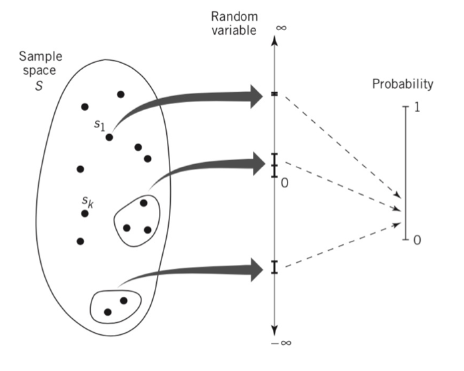
\includegraphics[width = 5cm]{media/insieme variabili aleatorie.png}
            \caption{Esperimento $\rightarrow$ Intervallo $\rightarrow$ Probabilitá dell'Intervallo}
        \end{figure}
        Una variabile aleatoria puó essere continua o discreta. Le variabil ialeatorie si indicano con le lettere
        maiuscole
        \subsubsection{Funzioni di Distribuzione - Distribution Functions}
            Considera la variabile aleatoria $X$ e la probabilitá dell'evento $X\leq x$, per convenzione si indica con $P[X\leq x]$,
            che puó essere scritto come:
            \[
                F_{X(x)} \triangleq P[X\leq x]\ \forall x    
            \]
            La funzione $F_{X(x)}$ é chiamata la \emph{funzione distribuzione} della variabile $X$, si puó notare che é funizone di $x$ non di 
            $X$.
            \paragraph{Propietá:}
                \begin{itemize}
                    \item {Limitata - Boundeness: é limitata tra zero e uno, essendo una probabilitá.}
                    \item {Monotona - Monotonicity: la funzione é una funzione monotona \emph{non decrescente} (puó rimanere costante) di $x$.}
                \end{itemize}
        \subsubsection{Funzione Densitá di Probabilitá - Probability Density Function (pdf)}
            La variabile aleatoria $X$ é continua se la funzione distribuzione $F_{X(x)}$ é differenziabile:
            \[
                f_{X(x)} = \derivative{}{x}F_{X(x)}\ \forall x    
            \]
            $f_{X(x)}$ é detta \emph{funzione di densitá di probabilitá} (pdf).
            \paragraph{Propietá:}
                \begin{itemize}
                    \item {Non negativa}
                    \item {Normalization: l'area totale della $pdf$ é unitaria.}
                    \item {
                        \begin{align}
                            P[x_1<X<x_2] &= P[X\leq x_2]  - P[X\leq x_1] = F_{X(x_2)} - F_{X(x_1)}  \nonumber \\
                                         &= \int_{x_1}^{x_2} f_{X(x)} dx\nonumber
                        \end{align}
                        se non avessi un estremo:
                        \begin{itemize}
                            \item {$ P[X\leq x_2] = \int_{-\infty}^{x_2}$}
                            \item {$ P[X\leq x_1] = 1-\int_{-\infty}^{x_1}$}
                        \end{itemize}
                    }
                \end{itemize}
            \paragraph{Esempio - Distribuzione Uniforme:} 
                Proviamo le propietá della funzione distribuzione $F_{X(x)}$ e la funzione densitá di probabilitá $f_{X(x)}$ per una variabile aleatoria
                continua:
                \[
                    f_{X(x)} = 
                    \begin{cases}
                        0 & x\leq a\nonumber \\
                        \frac{1}{b-a} & a<x\leq b\nonumber \\
                        0 & x>b\nonumber
                    \end{cases}  
                \]
                Integrandola troviamo:
                \[
                    F_{X(x)} = 
                    \begin{cases}
                        0 & x\leq a\nonumber \\
                        \frac{x-a}{b-a} & a<x\leq b\nonumber \\
                        1 & x>b\nonumber
                    \end{cases}  
                \]
                \begin{figure}[H]
                    \centering
                    \subfloat[$f_{X(x)}$]{
                        \begin{tikzpicture}
                            \begin{axis}[
                                xlabel=$x$,
                                ylabel=$f_{X(x)}$,
                                xmin=-0.2,
                                xmax=5,
                                ymin=-0.2,
                                ymax=2,
                                ytick = {1.5},
                                xtick={0, 1,2, 4},
                                xticklabels={$0$, $a$,$x_0$, $b$},
                                yticklabels = {$\frac{1}{b-a}$},
                                %yticklabel style = {yshift=5pt,xshift=4pt}, 
                                axis lines=middle,
                                thick,
                                domain=-4:4,
                                samples=100,
                                width=6.5cm,
                                height=4cm
                            ]
                        
                            \addplot [const plot, blue, thick] coordinates{(1,1.5)(4,1.5)};
                            \addplot [const plot, blue, thick] coordinates{(1,0)(1,1.5)};
                            \addplot [const plot, blue, thick] coordinates{(4,0)(4,1.5)};
                            \addplot [const plot, blue, thick] coordinates{(4,0)(5,0)};
                            \addplot [const plot, blue, thick] coordinates{(0,0)(1,0)};
                        
                            \addplot [const plot, blue, thin, name path = A] coordinates{(1,1.5)(2,1.5)};
                            \addplot [const plot, blue, thin, name path = B] coordinates{(1,0)(2,0)};
                        
                        
                            \addplot[red,opacity = 0.3] fill between[of=A and B];
                        


                            \end{axis}
                        \end{tikzpicture}
                    }
                    \hfill
                    \subfloat[$F_{X(x)}$]{
                        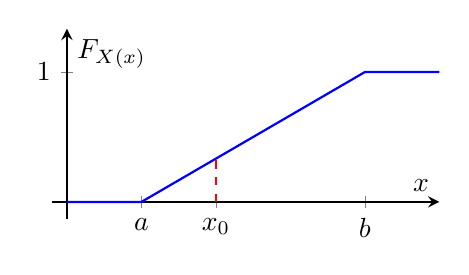
\begin{tikzpicture}
                            \begin{axis}[
                                xlabel=$x$,
                                ylabel=$F_{X(x)}$,
                                xmin=-0.2,
                                xmax=5,
                                ymin=-0.2,
                                ymax=2,
                                ytick = {1.5},
                                xtick={0, 1, 2,4},
                                xticklabels={$0$, $a$, $x_0$, $b$},
                                yticklabels = {$1$},
                                %yticklabel style = {yshift=5pt,xshift=4pt}, 
                                axis lines=middle,
                                thick,
                                domain=-5:5,
                                samples=100,
                                width=6.5cm,
                                height=4cm
                            ]
        
                            \addplot [sharp plot, blue, thick] coordinates{(0,0)(1,0)(4,1.5)(5,1.5)};
                            \addplot [dashed, red, thick] coordinates{(2,0)(2,0.5)};
        
                            \end{axis}
                        \end{tikzpicture}
                    }
                    \caption{Distribuzione Uniforme}
                    \label{Distribuzione Uniforme}
                \end{figure}
        \subsubsection{Funzione Probabilitá di massa - Probability Mass Function (pmf)}
            Consideriamo il caso di una variabile aleatoria discreta $X$, la quale puó assumere un numero rinito o infinito di valori. La funzione 
            distribuzione $F_{X(x)}$ si applica anche alle variabili discrete, ma non é differenziabile per come l'abbiamo definita. Definiamo 
            la funzione probabilitá di massa $p_{X(x)}$:
            \[
                p_{X(x)} \triangleq P[X = x]    
            \]
            é la probabilitá di un evento $X=x$, che consiste in tutti i possibili risultati di un esperimento i quali hanno un valore di 
            $X$ uguale a $x$.

            \paragraph{Esempio di Bernulli}
                Consideriamo l'esperimento probabilistico che assume uno di due valori:
                \begin{itemize}
                    \item {il valore 1 con probabilitá $p$}
                    \item {il valore 0 con probabilitá $1-p$}
                \end{itemize}
                Tale variabile aleatoria é chiamata \emph{variabile aleatoria di Bernulli}:
                \begin{figure}[H]
                    \centering
                    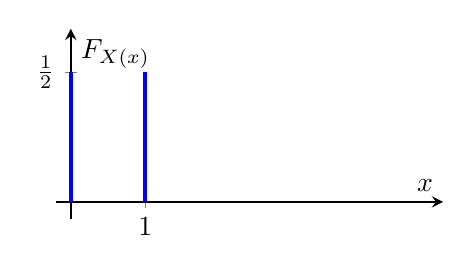
\begin{tikzpicture}
                        \begin{axis}[
                            xlabel=$x$,
                            ylabel=$F_{X(x)}$,
                            xmin=-0.2,
                            xmax=5,
                            ymin=-0.2,
                            ymax=2,
                            ytick = {1.5},
                            xtick={0, 1},
                            xticklabels={$0$, $1$},
                            yticklabels = {$\frac{1}{2}$},
                            %yticklabel style = {yshift=5pt,xshift=4pt}, 
                            axis lines=middle,
                            thick,
                            domain=-5:5,
                            samples=100,
                            width=6.5cm,
                            height=4cm
                        ]
    
                        \addplot [const plot, blue,ultra thick] coordinates{(0,0)(0,1.5)};
                        \addplot [const plot, blue,ultra thick] coordinates{(1,0)(1,1.5)};
    
                        \end{axis}
                    \end{tikzpicture}
                \end{figure}
        \subsubsection{ - Multiple Random Variables}
            Consideriamo due variabili aleatorie $X$ e $Y$:
            \begin{itemize}
                \item {
                    La funzione distribuzione $F_{X,Y (x,y)}$ é la probabilitá che $X$ sia minore o uguae a un valore specifico $x$ e che $Y$
                    sia minore o uguale a un'altro valore specifico $y$:
                    \[
                        F_{X,Y (x,y)} = P[X\leq x,Y\leq y]    
                    \]
                }
                \item {
                    La funzione densitá di probabilitá $f_{X,Y (x,y)}$ contiene tutto quello che ci serve per fare una completa analisi della probabilitá
                    di piú variabili aleatorie:
                    \[
                        f_{X,Y (x,y)} = \frac{d^2 F_{X,Y (x,y)}}{dxdy}     
                    \]

                }
            \end{itemize}
        \subsubsection{Funzione Densitá di Probabilitá Condizionata - Conditional Probability Density Function}
            Supponendo che $X$ e $Y$ siano due variabili aleatorie continue con $f_{X,Y (x,y)}$, la funzione densitá di probabilitá condizionata di $Y$ con $X=x$,
            é definita da:
            \[
                f_{Y (y|x)} = \frac{f_{X,Y (x,y)}}{f_{X(x)}}     
            \]
            Supponendo che le due variabili siano indipendenti: allora $f_{Y (y|x)}$ si riduce alla densitá marginale $f_{Y (y)}$ e la funzione densitá di
            probabilitá diventa $f_{X (x)}f_{Y (y)}$, se cosí fosse le due variabili si dicono \emph{statisticamente indipendenti}\index{Statisticamente Indipendenti}.
        \subsubsection{Somma di Variabili Aleatorie Indipendenti}
            Consideriamo due variabili aleatorie $X$ e $Y$ statisticamente indipendenti e continue con funzioni di densitá di probabilitá $f_{X (x)}$ e $f_{Y (y)}$ si 
            definisce $Z = X+Y$ la cui $pdf$ $f_{Z (z)}$ é:
            \[
                f_{Z (z)} = \int_{-\infty}^{\infty}f_{X (x)}f_{Y (z-y)} dx =  f_{X (x)} \otimes f_{Y (y)}
            \]
            La somma di due variabili aleatoria indipendeti e continue é la convoluzione delle funzioni di densitá di probabilitá.    
            Dimostrazione: (To DO: sul libro)
            \begin{figure}[H]
                \centering
                \subfloat[$f_{X(x)}$]{
                    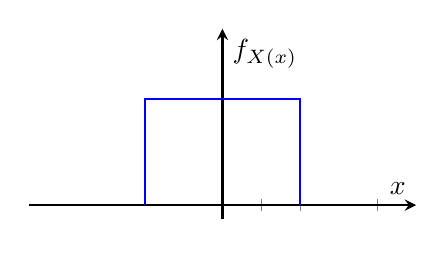
\begin{tikzpicture}
                        \begin{axis}[
                            xlabel=$x$,
                            ylabel=$f_{X(x)}$,
                            xmin=-5,
                            xmax=5,
                            ymin=-0.2,
                            ymax=2.5,
                            ytick = {1.5},
                            xtick={0, 1,2, 4},
                            xticklabels={},
                            yticklabels = {},
                            %yticklabel style = {yshift=5pt,xshift=4pt}, 
                            axis lines=middle,
                            thick,
                            domain=-5:5,
                            samples=100,
                            width=6.5cm,
                            height=4cm
                        ]
                        \addplot [const plot, blue, thick] coordinates{(-2,0)(-2,1.5)(2,1.5)(2,0)};
                        \end{axis}
                    \end{tikzpicture}
                }
                \hfill
                \subfloat[$f_{Y(y)}$]{
                    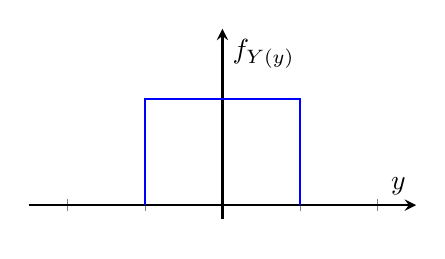
\begin{tikzpicture}
                        \begin{axis}[
                            xlabel=$y$,
                            ylabel=$f_{Y(y)}$,
                            xmin=-5,
                            xmax=5,
                            ymin=-0.2,
                            ymax=2.5,
                            ytick = {1.5},
                            xtick={},
                            xticklabels={},
                            yticklabels = {},
                            %yticklabel style = {yshift=5pt,xshift=4pt}, 
                            axis lines=middle,
                            thick,
                            domain=-5:5,
                            samples=100,
                            width=6.5cm,
                            height=4cm
                        ]
    
                        \addplot [const plot, blue, thick] coordinates{(-2,0)(-2,1.5)(2,1.5)(2,0)};
                        \end{axis}
                    \end{tikzpicture}
                }

                \subfloat[$f_{Z(z)}$]{
                    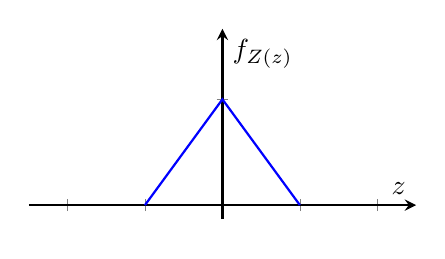
\begin{tikzpicture}
                        \begin{axis}[
                            xlabel=$z$,
                            ylabel=$f_{Z(z)}$,
                            xmin=-5,
                            xmax=5,
                            ymin=-0.2,
                            ymax=2.5,
                            ytick = {1.5},
                            xtick={},
                            xticklabels={},
                            yticklabels = {},
                            %yticklabel style = {yshift=5pt,xshift=4pt}, 
                            axis lines=middle,
                            thick,
                            domain=-5:5,
                            samples=100,
                            width=6.5cm,
                            height=4cm
                        ]
                        \addplot [sharp plot, blue, thick] coordinates{(-2,0)(0,1.5)(2,0)};
                        \end{axis}
                    \end{tikzpicture}
                }
                \caption{Somma di Variabili Aleatorie}
                \label{Somma di Variabili Aleatorie}
            \end{figure}
        \subsubsection{Valore medio delle Variabili Aleatorie - Mean Value of Random Variables (Expectation)}\label{Expectation}\index{Expectation}
            L'expectation o il valore medio di ua variabile aleatoria continua $X$ é formalemnte definito da:
            \begin{itemize}
                \item {Caso Continuo:
                    \[
                        \mu_X = \mathbb{E}[X] = \int_{-\infty}^{\infty} xf_{X(x)}dx
                    \]
                }
                \item {Caso Discreto:
                    \[
                        \mathbb{E}[X] = \sum_{x}xp_{X(x)}
                    \]
                }
            \end{itemize}
            é la media pesata delle variabili aleatorie, puó anche essere un valore che non gli appartiene.
            \paragraph{Propietá}
                \begin{itemize}
                    \item {\label{linearita expectation} Linearitá - Linearity: $\mathbb{E}[Z] = \mathbb{E}[X+Y]  = \mathbb{E}[X] +\mathbb{E}[Y]$.}
                    \item {\label{Indipendenza statistica}Indipendenza Statistica - Statistical Indipendence:$\mathbb{E}[Z] = \mathbb{E}[XY] = \mathbb{E}[X] \mathbb{E}[Y]$ 
                    se $X$ e $Y$ sono statisticamente indipendenti.\\
                    Dimostrazione:
                    \begin{align}
                        \mathbb{E}[XY] &= \int_{-\infty}^{\infty}\int_{-\infty}^{\infty} xy f_{X,Y (x,y)} dxdy \overset{Indipendenza}{=} \int_{-\infty}^{\infty}\int_{-\infty}^{\infty} xy f_{X (x)}f_{Y (y)} dxdy \nonumber \\
                                       &= E[X]E[Y] \nonumber
                    \end{align}
                    }
                    \item {\label{valor medio expectation} Teorema del valore medio dell'expectation: 
                        \[
                            \mathbb{E}[g_{(x)}] \overset{Y=g_{(x)}}{=} \mathbb{E}[Y] =  \int_{-\infty}^{\infty}yf_{Y(y)}dy \triangleq \int_{-\infty}^{\infty}g_{(x)}f_{X(x)}dx
                        \]
                    }
                \end{itemize}
            \paragraph{Esempi:}\label{esempi expectation}
                \begin{enumerate}
                    \item{
                        Calcolare il valore medio ($\mu_X$) di:
                        \begin{figure}[H]
                            \centering
                            \begin{tikzpicture}
                                \begin{axis}[
                                    xlabel=$x$,
                                    ylabel=$f_{X(x)}$,
                                    xmin=-0.2,
                                    xmax=5,
                                    ymin=-0.2,
                                    ymax=2.5,
                                    ytick = {1.5},
                                    xtick={1,3},
                                    xticklabels={$a$,$b$},
                                    yticklabels = {$\frac{1}{b-a}$},
                                    axis lines=middle,
                                    domain=0:5,
                                    samples=100,
                                    width=6.5cm,
                                    height=4cm
                                ]
                                \addplot [const plot, blue, thick] coordinates{(1,0)(1,1.5)(3,1.5)(3,0)};
                                \end{axis}
                            \end{tikzpicture}
                        \end{figure}

                        \begin{align}
                            \mu_X &= \int_{-\infty}^{\infty}xf_{X(x)}dx = \int_{a}^{b}\frac{x}{b-a}dx = \eval{\frac{x^2}{2(b-a)}}_{a}^{b}\nonumber \\
                                  &= \frac{b^2-a^2}{2(b-a)} = \frac{b+a}{2}\nonumber 
                        \end{align}
                    }
                    \item{
                        Calcoliamo il valore quadratico medio della distribuzione unitaria ($\mathbb{E}[x^2]$):
                        \begin{align}
                            \mathbb{E}[X^2] &= \int_{-\infty}^{\infty}x^2f_{X(x)}dx = \int_{a}^{b}\frac{x^2}{b-a}dx = \eval{\frac{x^3}{3(b-a)}}_{a}^{b}\nonumber \\
                                            &= \frac{b^3-a^3}{3(b-a)} = \frac{b^2+ab+a^2}{3}\nonumber 
                        \end{align}
                    }
                \end{enumerate}
        \subsubsection{Varianza - Variance}
            La varianza $\sigma^2_x$ di una variabile aleatoria $X$ é definita:
            \[
                var[X] = \mathbb{E}[(X-\mu_X)^2] = \int_{-\infty}^{\infty} (X-\mu_X)^2f_{X(x)}dx
            \]  
            \begin{align}
                var[X] &= \sigma^2_x \overset{\ref{linearita expectation}}{=} \mathbb{E}[X^2-2\mu_XX+\mu_X^2] = \mathbb{E}[X^2]-2\mu_X\mathbb{E}[X]+\mu_X^2 \nonumber \\
                           &= \mathbb{E}[X^2]-\mu_X^2 \nonumber 
            \end{align}\index{Valore quadratico medio}
            $\mathbb{E}[X] = \int_{-\infty}^{\infty} xf_{X(x)}dx$ mentre $\mathbb{E}[X^2] = \int_{-\infty}^{\infty} x^2f_{X(x)}dx$, l'expectation é il peso che diamo alla funzione $f_{X(x)}$.  
            Misura la "randomicitá" di una variabile aleatoria, meno é randomica piú sono vicino al mio valor medio.
            \[
                P[|X-\mu_X|\geq \mathcal{E}]\leq \frac{\sigma^2_X}{\mathcal{E}^2}
            \]
            \paragraph{Deviazione Standard:} $\sigma_X = \sqrt[2]{\sigma^2_X}$ si dice Deviazione Standard
        \subsubsection{Covarianza - Covariance}
            Siano $X$ e $Y$ due variabili aleatorie, si definisce covarianza:
            \begin{gather}
                cov[XY] = \mathbb{E}[(X-\mathbb{E}[X])(Y-\mathbb{E}[Y])]\nonumber\\
                = \mathbb{E}[XY]-\mu_X\mu_Y\nonumber
            \end{gather}
            Il \emph{coefficiente di correlazione}\index{Coefficiente di Correlazione} di $X$ e $Y$ é:
            \[
                \rho_{(X,Y)} = \frac{cov[XY]}{\sigma_X\sigma_Y}
            \]
            misura la somiglianza tra $X$ e $Y$. Le due variabili si dicono:
            \begin{itemize}
                \item {
                    Incorrelate: se la $cov[XY] =0$, ció non implica l'indipendenza delle variabili.
                }
                \item {
                    Ortogonali: se $\mathbb{E}[XY] = 0$
                }
            \end{itemize}
        \subsubsection{Distribuzione Gaussiana}
            \begin{figure}[H]
                \centering
                    \begin{tikzpicture}
                        \begin{axis}[
                            xlabel=$x$,
                            ylabel=$f_{X(x)}$,
                            xmin=-5,
                            xmax=5,
                            ymin=-0.2,
                            ymax=0.8,
                            xtick={},
                            yticklabel style = {font = \scriptsize}, 
                            xticklabels={},
                            axis lines=middle,
                            domain=-5:5,
                            width=12cm,
                            height=5cm
                        ]
                        \addplot [const plot, blue, thick, samples = 500] {gauss(0,0.7)};
                        \end{axis}
                    \end{tikzpicture}
                \caption{Gaussiana}
            \end{figure}               
            Una variabile aleatoria $X$ é detta Gaussiana se la funzione distribuzione di probabilitá ,$pdf$, ha la forma:
            \[
                f_{X(x)} = \frac{1}{\sqrt{2\pi}\sigma_X}e^{\left[\displaystyle -\frac{(x-\mu_X)^2}{2\sigma^2_X}\right]}  
            \]
            \paragraph{Propietá:}\label{propieta distr gaussiana}
            \begin{itemize}
                \item {Definita unicamente da valore medio di $X$ e la varianza $\mathcal{N}(\mu_X,\sigma_X^2)$.}
                \item {\begin{sloppypar}
                    La propietá di Gaussianitá é preservata dalle trasformazioni lineari. ${X \sim \mathcal{N}(\mu_X,\sigma_X^2): Y = \alpha X+\beta}$, calcoliamo come variano 
                    valor medio e varianza:
                \end{sloppypar}
                    \begin{itemize}
                        \item {Valor medio:
                            \[
                                \mathbb{E}[Y] = \mu_Y = \mathbb{E}[\alpha X+\beta]  \overset{\ref{linearita expectation}}{=} \alpha \mathbb{E}[X] + \beta
                            \]
                        }
                        \item {Varianza:
                            \begin{align}
                                \sigma_Y^2  &= \mathbb{E}[Y^2] -\mathbb{E}[Y]^2 =\mathbb{E}[(\alpha X + \beta)^2] -(\alpha \mathbb{E}[X] + \beta)^2 \nonumber \\
                                            &= \mathbb{E}[\alpha^2 X^2 + \beta^2 +2\alpha\beta X] -(\alpha^2 \mathbb{E}[X]^2 + \beta^2 +2\alpha\beta\mathbb{E}[X])\nonumber \\
                                            &= \alpha^2 \mathbb{E}[X^2] + \beta^2 +2\alpha\beta \mathbb{E}[X] -\alpha^2 \mathbb{E}[X]^2 - \beta^2 -2\alpha\beta\mathbb{E}[X]\nonumber \\
                                            &= \alpha^2 \mathbb{E}[X^2] -\alpha^2 \mathbb{E}[X]^2 = \alpha^2 (\mathbb{E}[X^2] -\mathbb{E}[X]^2)\nonumber \\
                                            &= \alpha^2 (\mathbb{E}[X^2] -\mu_X^2)=\alpha^2 \sigma_X^2\nonumber
                            \end{align}                         
                            la costante $\beta$ non influisce la varianza.  
                        }
                    \end{itemize}}
                \item {La somma $Z = X+Y$ di variabili aleatorie Gaussiane indipendenti é anche essa na variabile aleatoria
                    Gaussiana, con:
                        \begin{itemize}
                            \item {$\mathbb{E}[Z] = \mathbb{E}[X] +\mathbb{E}[Y] $}
                            \item {$var[Z] = var[X] +var[Y] $}
                        \end{itemize}}
            \end{itemize}
            \paragraph{Distribuzione Gaussiana Standard}
                Si dice forma Gaussiana Standard se: $\mathbb{E}[X] = 0$ e $var[X] = 1$, $\mathcal{N}(0,1)$:
                \begin{gather}
                    f_{X(x)} = \frac{1}{\sqrt{2\pi}} e^{\displaystyle\left(-\frac{x^2}{2}\right)}\nonumber \\
                    F_{X(x)} =P[X\leq x] = \int_{-\infty}^{\infty}f_{X(x)} =\frac{1}{\sqrt{2\pi}} \int_{-\infty}^{x}e^{\displaystyle\left(-\frac{t^2}{2}dt\right)}\nonumber 
                \end{gather}

                \begin{figure}[H]
                    \centering
                    \subfloat[$f_{X(x)}$]{
                        \begin{tikzpicture}
                            \begin{axis}[
                                xlabel=$x$,
                                ylabel=$f_{X(x)}$,
                                xmin=-5,
                                xmax=5,
                                ymin=-0.2,
                                ymax=0.8,
                                xtick={},
                                yticklabel style = {font = \scriptsize}, 
                                xticklabels={},
                                axis lines=middle,
                                domain=-5:5,
                                samples=100,
                                width=6.5cm,
                                height=5cm
                            ]
                            \addplot [const plot, blue, thick, samples = 300] {gauss(0,1)};
                            \end{axis}
                        \end{tikzpicture}
                    }
                    \hfill
                    \subfloat[$F_{X(x)}$]{
                        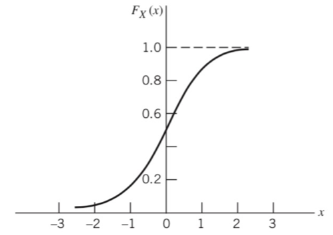
\includegraphics[width = 6cm]{media/funzione distribuzione gaussiana.png}
                    }
                    \caption{Distribuzione Gaussiana Standard}
                \end{figure}
                Osservazioni: la varianza permette di modificare la spanciatura della gaussiana, mentre il valor medio shifta sull'asse x la gaussiana.

                Posso utilizzare la forma standard della gaussiana e le trasformazioni lineari per rappresentare qualsiasi altro tipo di gaussiana:
                \[
                    Y\sim \mathcal{N}(\mu_y,\sigma_Y^2) \rightarrow Y = \sigma_Y X + \mu_y
                \]
                Calcoliamo $\mu_Y$ e $\sigma_Y^2$:
                \begin{itemize}
                    \item {$\mathbb{E}[Y] = \mu_Y$}
                    \item {$\sigma_Y^2 = \sigma_X^2 \sigma_Y^2 $}
                \end{itemize}
        \subsubsection{Funzione $Q_{(x)}$}
            Per calacolare la funzione distribuzione di probabilitá ($F_{X(x)}$) non calcoliamo l'integrale della funzione distribuzione di probabilitá, 
            ma utilizziamo la funzione $Q_{(x)}$ cosí definita:
            \[
                Q_{(x)} = 1-F_{X(x)} = P[X\geq x]  
            \]
            formalmente é cosi definita:
            \[
                Q_{(x)} = 1-F_{X(x)} = 1 - \frac{1}{\sqrt{2\pi}} \int_{-\infty}^{x}e^{\left(-\frac{t^2}{2}dt\right)} = \frac{1}{\sqrt{2\pi}} \int_{x}^{\infty}e^{\left(-\frac{t^2}{2}dt\right)}  
            \]
            é l'area sottesa dalla funzione di distribuzione Gaussiana da $x$ all'infinito

            \begin{figure}[H]
                \centering
                \subfloat[$f_{X(x)}$]{
                    \begin{tikzpicture}
                        \begin{axis}[
                            xlabel=$x$,
                            ylabel=$f_{X(x)}$,
                            xmin=-5,
                            xmax=5,
                            ymin=-0.2,
                            ymax=0.8,
                            xtick={1},
                            yticklabel style = {font = \scriptsize}, 
                            xticklabels={$x$},
                            axis lines=middle,
                            domain=-5:5,
                            samples=100,
                            width=7cm,
                            height=5cm
                        ]
                        \addplot [const plot, blue, thick, samples = 300] {gauss(0,1)};
                        \addplot [const plot, blue,name path = A, thick, samples = 300, domain = 1:5] {gauss(0,1)};
                        \addplot [const plot, black,name path = B, thin] coordinates{(1,0)(5,0)};

                        \addplot[red,opacity = 0.3] fill between[of=A and B];
                        \end{axis}
                    \end{tikzpicture}
                }
                \caption{\color{red}$Q_{(x)}$}
            \end{figure}
            \paragraph{Propietá:}
            \begin{itemize}
                \item {$Q_{(x)} = 1-Q_{(-x)}$

                        \begin{figure}[H]
                            \centering
                                \begin{tikzpicture}
                                    \begin{axis}[
                                        xlabel=$x$,
                                        ylabel=$f_{X(x)}$,
                                        xmin=-5,
                                        xmax=5,
                                        ymin=-0.2,
                                        ymax=0.8,
                                        xtick={-1,1},
                                        yticklabel style = {font = \scriptsize}, 
                                        xticklabels={$-x$,$x$},
                                        axis lines=middle,
                                        domain=-5:5,
                                        samples=100,
                                        width=7cm,
                                        height=5cm
                                    ]
                                    \addplot [const plot, blue, thick, samples = 300] {gauss(0,1)};
                                    \addplot [const plot, blue,name path = A, thick, samples = 300, domain = 1:5] {gauss(0,1)};
                                    \addplot [const plot, black,name path = B, thin] coordinates{(1,0)(5,0)};
                                    \addplot [const plot, blue,name path = C, thick, samples = 300, domain = -5:-1] {gauss(0,1)};
                                    \addplot [const plot, black,name path = D, thin] coordinates{(-5,0)(-1,0)};

                                    \addplot[red,opacity = 0.3] fill between[of=A and B];
                                    \addplot[yellow,opacity = 0.3] fill between[of=C and D];
                                    \end{axis}
                                \end{tikzpicture}
                            
                            \caption{{\color{red}$Q_{(x)}$},{\color{yellow}$1-Q_{(-x)}$}}
                        \end{figure}
                }
                \item {$Q_{(\infty)} = 0$}
                \item {$Q_{(-\infty)} = 1$}
                \item {$Q_{(0)} = \frac{1}{2}$}
            \end{itemize}
            utilizziamo la tavola della funzione $Q$
            \begin{figure}[H]
                \centering
                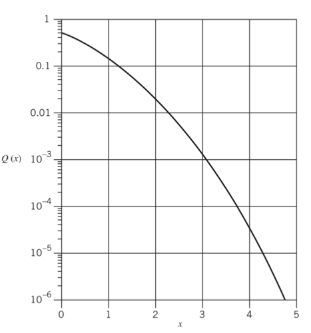
\includegraphics[width = 8cm]{media/grafo funzione q.png}
                \caption{Grafico $Q_{(x)}$}
            \end{figure}
        \subsubsection{Teorema del Limite Centrale - Central Limit Theorem}\label{Teorema del Limite Centrale - Central Limit Theorem}
            Siano $X_1,\dots,X_n$ una sequenza di variabili aleatorie indipendenti e identicamente distribuite con valore medio $\mu$ e varianza $\sigma$:
            \[
                Y_n = \frac{1}{\sigma\sqrt{n}}\left(\sum_{i=1}^{n}X_i-n\mu\right)    
            \]
            al tendere di $n$ all'infinito, $Y_n$ converge alla variabile aleatoria Gaussiana standard:
            \[
                F_{Y(y)} =P[Y\leq y] = \frac{1}{\sqrt{2\pi}} \int_{-\infty}^{y}e^{\left(-\frac{x^2}{2}dx\right)}    
            \]
        \subsubsection{Calcolo probabilitá di errore di un sistema} 
            Dato un sistema binario di comunicazione ($S\in\{0,1\}$), dopo il campionamento ho: $Y = \sqrt{p}S+n$. $p$ é la potenza e $n$ é il rumore
            gaussiano $n \sim \mathcal{N}(0,\sigma_n^2)$. Voglio calcolarne la probabilitá di errore:
            \[
                P_e \overset{\ref{Legge della probabilitá totale}}{=} P_r(\hat{S}=1|S=-1)P(S=-1)+ P_r(\hat{S}=-1|S=1)P(S=1)   
            \] 
            \begin{sloppypar}
                \noindent analizziamo il caso generico in cui ${P(S=1) = q, P(S=-1)=1-q}$, nel caso equiprobabile sarebbero $\frac{1}{2}$: dobbiamo calcolare 
                ${P_r(\hat{S}=1|S=-1)}$ e ${P_r(\hat{S}=-1|S=1)}$
            \end{sloppypar}
            \begin{itemize}
                \item {$P_r(\hat{S}=1|S=-1)$:
                    \[
                        \eval*{Y}_{S = -1} = -\sqrt{p}+n \sim \mathcal{N}(-\sqrt{p},\sigma_Y = \sigma_n^2)  
                    \]
                    al rumore viene solo aggiunta una costante, quindi rimane tale e con distribuzione:
                    \begin{figure}[H]
                        \centering
                            \begin{tikzpicture}
                                \begin{axis}[
                                    xlabel=$x$,
                                    ylabel=$f_{X(x)}$,
                                    xmin=-10,
                                    xmax=10,
                                    ymin=-0.2,
                                    ymax=0.8,
                                    xtick={-1},
                                    yticklabel style = {font = \scriptsize}, 
                                    xticklabels={$-\sqrt{p}$},
                                    axis lines=middle,
                                    domain=-7:7,
                                    width=12cm,
                                    height=5cm
                                ]
                                \addplot [const plot, blue, thick, samples = 500] {gauss(-1,1)};
                                \addplot [const plot, blue, name path = A,thick, samples = 500, domain = 0:5] {gauss(-1,1)};
                                \addplot [const plot, black,name path = B, thin] coordinates{(0,0)(5,0)};

                                \addplot[red,opacity = 0.3] fill between[of=A and B];
                                \end{axis}
                            \end{tikzpicture}
                        \caption{{\color{red}$P[Y\geq 0|S=-1]$}}
                    \end{figure}                    
                    posso basare la decisione di errore se ricevo qualcosa di positivo quando il simbolo inviato é negativo, $P[Y\geq 0|S=-1]$.
                    
                    \paragraph{Calcolo errore di un sistema:} Posso generalizzare la mia soglia di decisione su di un valore $\lambda$ 
                    \begin{figure}[H]
                        \centering
                            \begin{tikzpicture}
                                \begin{axis}[
                                    xlabel=$x$,
                                    ylabel=$f_{X(x)}$,
                                    xmin=-10,
                                    xmax=10,
                                    ymin=-0.2,
                                    ymax=0.8,
                                    xtick={-1,0.5},
                                    yticklabel style = {font = \scriptsize}, 
                                    xticklabels={$-\sqrt{p}$,$\lambda$},
                                    axis lines=middle,
                                    domain=-7:7,
                                    width=12cm,
                                    height=5cm
                                ]
                                \addplot [const plot, blue, thick, samples = 500] {gauss(-1,1)};
                                \addplot [const plot, blue, name path = A,thick, samples = 500, domain = 0.5:5] {gauss(-1,1)};
                                \addplot [const plot, black,name path = B, thin] coordinates{(0.5,0)(5,0)};

                                \addplot[red,opacity = 0.3] fill between[of=A and B];
                                \end{axis}
                            \end{tikzpicture}
                        \caption{{\color{red}$P[Y\geq \lambda|S=-1]$}}
                    \end{figure}               
                    di conseguenza la probabilitá viene descritta come:
                    \[
                        P_r[\hat{S} = 1|S=-1] = P_r[Y> \lambda|S=-1] = P_r[-\sqrt{p}+n > \lambda] =P_r[n > \lambda+\sqrt{p}]
                    \]
                    posso calcolare la $P_r[-\sqrt{p}+n > \lambda]$ oppure $P_r[n > \lambda+\sqrt{p}]$, calcoliamo $P_r[n > \lambda+\sqrt{p}]$:
                    \begin{align}
                        Q_{(x)} &= \int_{x}^{\infty} \frac{1}{\sqrt{2\pi}} e^{-\frac{t^2}{2}}dt\nonumber \\
                                &= \int_{\lambda+\sqrt{p}}^{\infty}f_{N(n)}dn\text{ senza sapere se é gaussiana o meno}\nonumber \\
                                &\overset{\text{é Gaussiana}}{=} \int_{\lambda+\sqrt{p}}^{\infty}\frac{1}{\sqrt{2\pi}\sigma_n}e^{-\frac{n^2}{2\sigma_n^2}}dn \overunderset{t = \frac{n}{\sigma_n}}{dt = \frac{dn}{\sigma_n}}{=} \int_{\frac{\lambda+\sqrt{p}}{\sigma_n}}^{\infty}\frac{1}{\sqrt{2\pi}}e^{-\frac{t^2}{2}}dt\nonumber \\
                                &= Q_{\left(\frac{\lambda +\sqrt{p}}{\sigma_n}\right)} = P_r[n>\lambda + \sqrt{p}]\nonumber 
                    \end{align}
                    generalizzando la potenza del segnale ottengo l'errore\index{Errore Gaussiano}:
                    \[
                        Q_{\displaystyle\left(\frac{\lambda -\mu_Y}{\sigma_Y}\right)} = P_r[n>\lambda + \mu_Y]
                    \]
                }
                \item {Calcoliamo ${P_r(\hat{S}=-1|S=1)}$ applicando la formula dell'errore sopra trovata:
                    \[
                        S=1\Rightarrow Y = \sqrt{p}+n\sim\mathcal{N}(\sqrt{p},\sigma_n^2)  
                    \]
                    calcolando la probabilitá:
                    \begin{align}
                        P_r[\hat{S}=-1|S=1] &= 1-P_r[\hat{S}=1|S=-1] = 1- Q_{\displaystyle\left(\frac{\lambda -\mu_Y}{\sigma_Y}\right)}  \nonumber \\
                                            &= 1- Q_{\displaystyle\left(\frac{\lambda -\sqrt{p}}{\sigma_n}\right)}\nonumber
                    \end{align}
                    sottraggo a $1$ la probabilitá per la definizione della $Q_{(x)}$ é l'integrale della zona a dx e a me interessa l'area a sinistra:
                    \begin{figure}[H]
                        \centering
                            \begin{tikzpicture}
                                \begin{axis}[
                                    xlabel=$x$,
                                    ylabel=$f_{X(x)}$,
                                    xmin=-10,
                                    xmax=10,
                                    ymin=-0.2,
                                    ymax=0.8,
                                    xtick={1},
                                    yticklabel style = {font = \scriptsize}, 
                                    xticklabels={$\sqrt{p}$},
                                    axis lines=middle,
                                    domain=-7:7,
                                    width=12cm,
                                    height=5cm
                                ]
                                \addplot [const plot, blue, thick, samples = 500] {gauss(1,1)};
                                \addplot [const plot, blue, name path = A,thick, samples = 500, domain = -5:0] {gauss(1,1)};
                                \addplot [const plot, black,name path = B, thin] coordinates{(-0,0)(-5,0)};

                                \addplot[red,opacity = 0.3] fill between[of=A and B];
                                \end{axis}
                            \end{tikzpicture}
                        \caption{{\color{red}$P[\hat{S}=-1|S=1]$}}
                    \end{figure}               
                }
            \end{itemize}
            La probabilitá totale di errore del sistema é:
            \begin{align}
                P_e &= Q_{\displaystyle\left(\frac{\lambda +\sqrt{p}}{\sigma_n}\right)} P[S=-1]+\left(1- Q_{\displaystyle\left(\frac{\lambda -\sqrt{p}}{\sigma_n}\right)}\right)P[S=1]\nonumber \\
                    &= Q_{\displaystyle\left(\frac{\lambda +\sqrt{p}}{\sigma_n}\right)} (1-q)+\left(1- Q_{\displaystyle\left(\frac{\lambda -\sqrt{p}}{\sigma_n}\right)}\right)q = g_{(\lambda)}\nonumber \\
            \end{align}
            se volessi calcolare il $\lambda$ ottimo derivo la funzione e la pongo uguale a zero: $\derivative{}{\lambda}g_{(\lambda)}=0$
            \paragraph{Caso con simboli equiprobabili:} $q=\frac{1}{2},\ \lambda = 0$
                \begin{align}
                    P_e &= \frac{1}{2}Q_{\left(\frac{\sqrt{p}}{\sigma_n}\right)}+ \frac{1}{2}\left(1-Q_{\left(\frac{\sqrt{p}}{\sigma_n}\right)}\right)\nonumber \\
                        &\overset{Q_{x} = 1-Q_{(-x)}}{=} Q_{\left(\frac{\sqrt{p}}{\sigma_n}\right)} = Q_{(\sqrt{SNR})}\nonumber  
                \end{align}
                si definisce $SNR\ =\ Signal\ To\ Noise\ Ratio =\frac{\mu^2}{\sigma_n^2}$ é il rapporto tra potenza e varianza, in generale caloclo:
                \[
                    Z = \frac{Y}{\sqrt{p}} = S+\frac{n}{\sqrt{p}} \sim \mathcal{N}(\pm 1,\frac{\sigma_n^2}{p})   
                \] 
                da cui calcolandone la probabilitá di errore:
                \[
                    P_e = Q_{\left(\frac{1}{\sigma_n}\right)} = Q_{\left(\sqrt{\frac{p}{\sigma_n^2}}\right)}
                \]
                \subparagraph*{Esempio:} Ho bisogno di una $P_e = 10^{-3}$, quale rapporto $SNR$ devo utilizzare?
                \[
                    Q_{\sqrt{SNR}} = 10^{-3}   
                \]
                Controllando la tabella della funzione $Q_{(x)}$:
                \[
                    \sqrt{SNR} = 3 \Rightarrow SNR=9    
                \]
                Passando alla scala in decibel:
                \[
                    \eval*{SNR}_{db} = 10 \log_{10}(9) = 9.5db    
                \]
            \paragraph{Caso con rumore complesso:} $Y = \sqrt{p}S + n$:
                \begin{gather}
                    n\sim \mathcal{N}_c(0,\sigma_n^2)\rightarrow n = n_{Re} + jN_{Im} \nonumber \\
                    n_{Re},n_{Im}\sim \mathcal{N}_c(0,\frac{\sigma_n^2}{2})\nonumber
                \end{gather}
                Verifichiamo che la varianza delle singole componenti reali e immaginarie sia giusta:
                \[
                    var[n] = \mathbb{E}[|n|^2]-\mu_n^2 = var[n_{Re}]+ var[n_{Im}] = \frac{\sigma_n^2}{2} + \frac{\sigma_n^2}{2} = \sigma_n^2
                \]
                il procedimento  é uguale escludiamo la parte immaginaria del rumore e prendiamo solo quella reale (cambia solo il valore della varianza),
                poiché il simbolo ha solo parti reali:
                \[
                    Y \in \mathbb{C} 
                    \begin{cases}
                        Re\{Y\} = Y_{Re} = \sqrt{p}S_{Re} + n_{Re}\nonumber \\
                        Im\{Y\} = Y_{Im} = n_{Im}\nonumber    
                    \end{cases}      
                \]      
                e baso la mia decisione del simbolo ricevuto solo con la parte reale:
                \[
                    \hat{S} = 
                    \begin{cases}
                        1 &Re\{Y\} \geq\lambda\nonumber \\    
                        -1 &Re\{Y\} <\lambda\nonumber    
                    \end{cases}  = 
                    \begin{cases}
                        1 &Re\{Y\} \geq0\nonumber \\    
                        -1 &Re\{Y\} <0\nonumber    
                    \end{cases}    
                \]
                calcoliamo la probabilitá di errore:
                \begin{align}
                    Z_r &= \frac{Y_{Re}}{\sqrt{p}} = S+ \frac{n}{\sqrt{p}} \sim \mathcal{N}(0,\sigma^2):\ \sigma^2 = \frac{\sigma^2_n}{2p}\nonumber \\
                    P_e &= Q_{\displaystyle\left(\frac{1}{\sigma}\right)} = Q_{\displaystyle\left(\sqrt{\frac{2p}{\sigma_n^2}}\right)} = Q_{\sqrt{2SNR}}\nonumber
                \end{align}
                se $P_e = 10^{-3}$:
                \[
                    SNR = 4,5\overset{db}{\Rightarrow}{SNR}_{db}=6,53db    
                \]

                se $P_e = 10^{-5}$:
                \[
                    SNR = 8\overset{db}{\Rightarrow}{SNR}_{db}=9,03db    
                \]
                Nel caso del rumore complesso ho solo metá del distudbo dovuto ad esso poiché il simbolo non dipende dalla parte immaginaria.
            \paragraph{Caso con rumore e simboli complessi:} $Y = \sqrt{p}S + n \sim \mathcal{N}(0,\sigma_n^2)$:
                \[
                    Y \in \mathbb{C} 
                    \begin{cases}
                        Re\{Y\} = Y_{Re} = \sqrt{p}S_{Re} + n_{Re}\nonumber \\
                        Im\{Y\} = Y_{Im} = \sqrt{p}S_{Im} + n_{Im}\nonumber    
                    \end{cases}  
                \]
                \begin{figure}[H]
                    \centering
                        \begin{tikzpicture}
                            \begin{axis}[
                                xlabel=$Re$,
                                ylabel=$Im$,
                                xmin=-5,
                                xmax=5,
                                ymin=-5,
                                ymax=5,
                                xtick={},
                                xticklabels={},
                                yticklabels={},
                                axis lines=middle,
                                domain=-7:7,
                                width=8cm,
                                height=8cm
                            ]
                            \addplot+[only marks,
                            point meta=explicit symbolic,
                            nodes near coords,
                            every node near coord/.style={anchor=180}] % adjust anchor to your liking
                            coordinates {
                              (2.5,2.5) [$1+j$]
                              (-2.5,2.5) [$-1+j$]
                              (-2.5,-2.5) [$-1-j$]
                              (2.5,-2.5) [$1-j$]
                            };
                            \end{axis}
                        \end{tikzpicture}
                    \caption{Simboli complessi}
                \end{figure}
                basiamo la decisione del simbolo ricevuto rispetto al quadrante in cui cade, la probabiltiá di errore del 
                sistema $P_e$ é costituita dalla probabiltiá di scegliere un quadrante del simbolo diverso da quello inviato:
                \[
                    P_e = \sum_{k=1}^{4} P_r[\hat{S} \neq S_k | S_k]P[S_k]
                \]
                si noti come la probabilitá che il simbolo ricada in un quadrante diverso da quello inviato é identica per tutti i casi, 
                quindi basta calcolarne solo una: 
                \[
                    P_e = P_r[\hat{S} \neq S_1 | S=S_1]\sum_{k=1}^{4} P[S_k] = P_r[\hat{S} \neq S_1 | S=S_1]
                \]
                la somma delle probabilitá di trasmissione dei simboli é $1$, diventa praticamente la probabilitá di aver trasmesso un simbolo e quello lo faccio sempre.
                Calcoliamo $P_r[\hat{S} \neq S_1 | S=S_1]$:
                \[
                    P_r[\hat{S} \neq S_1 | S=S_1] \overset{P[corr. ricezione]}{=} 1-P_r[\hat{S} = S_1 | S=S_1] = 1-P_r[Y_{Re},Y_{Im} \in I^o ] 
                \]
                la parte reale e immaginaria sono tra loro indipendenti e gaussiane data la composizione del rumore $n$, posso calcolare:
                \[
                    P_r[Y_{Re},Y_{Im} \in I^o ] = P_r[Y_{Re}>0]P_r[Y_{Im}>0] 
                \]
                dall'esercizio sopra con rumore e simboli reali sappiamo che la probabilitá di corretta ricezione é $1-Q_{(\sqrt{2SNR})}$:
                \[
                    P_r[Y_{Re},Y_{Im} \in I^o ] = P_r[Y_{Re}>0]P_r[Y_{Im}>0] = \left(1-Q_{(\sqrt{2SNR})}\right)^2
                \]
                possiamo calcolare adesso la probabilitá del sistema:
                \begin{gather}
                    P_e = 1-\left(1-Q_{(\sqrt{2SNR})}\right)^2 =1-\left(1-2Q_{(\sqrt{2SNR})}+Q^2_{(\sqrt{2SNR})}\right)^2  \nonumber\\
                        = 2Q_{(\sqrt{2SNR})}-Q^2_{(\sqrt{2SNR})} \backsimeq 2Q_{(\sqrt{2SNR})}\nonumber
                \end{gather}
                il risultato é l'applicazione del secondo assioma in caso di eventi non disgiunti (\ref{Ass. Prob. 2}):
                \[    
                    \underset{P[A\cap B]}{\underbrace{P_e }}=\underset{P[A]+P[B]}{\underbrace{2Q_{(\sqrt{2SNR})}}}-\underset{-P[A\cup B]}{\underbrace{Q^2_{(\sqrt{2SNR})}}} 
                \]
                
          
    